\documentclass[a4paper]{article}

%use the english line for english reports
\usepackage[english]{babel}
\usepackage[utf8]{inputenc}
\usepackage{indentfirst}
\usepackage{graphicx}
\usepackage{verbatim}
\usepackage{minted}

\begin{document}

\setlength{\textwidth}{16cm}
\setlength{\textheight}{22cm}

\title{\Huge\textbf{Azacru}\linebreak\linebreak\linebreak
\Large\textbf{Final Report}\linebreak\linebreak
\linebreak\linebreak

\includegraphics[scale=0.1]{feup-logo.png}\linebreak\linebreak
\linebreak\linebreak
\Large{Mestrado Integrado em Engenharia Informática e Computação} \linebreak\linebreak
\Large{Programação em Lógica}\linebreak
}

\author{\textbf{Grupo Azacru\_2:}\\ David Falcão - up201506571 \\ Pedro Miranda - up201506574 \\\linebreak\linebreak \\
 \\ Faculdade de Engenharia da Universidade do Porto \\ Rua Roberto Frias, s\/n, 4200-465 Porto, Portugal \linebreak\linebreak\linebreak
\linebreak\linebreak\vspace{1cm}}
%\date{Junho de 2007}
\maketitle
\thispagestyle{empty}

%************************************************************************************************
%************************************************************************************************

\newpage

\section*{Summary}
This project consists of the implementation in Prolog of Azacru, a board game created in 2005.

We implement all functionalities of the game, always thinking on thinking of building the simplest solution possible for the given goal. 

Despite we already have contact with Prolog at classes, this project was the 'real introduction' to this language, so this was the main difficulty along all work but that we overcame with success.


\newpage

\tableofcontents

%************************************************************************************************
%************************************************************************************************

%*************************************************************************************************
%************************************************************************************************

\newpage

%%%%%%%%%%%%%%%%%%%%%%%%%%
\section{Introduction}
This project was developed within the scope of the 'Programação em Lógica' course of the 3rd year of MIEIC at the University of Porto. The objective was develop a game in Prolog.

Although this game wasn't our first choice, we saw this project as a challenge and interpret knowledge acquired in Prolog as a reward.



\vspace{10mm}
%%%%%%%%%%%%%%%%%%%%%%%%%%
\section{The Game Azacru}

\subsection{History}
In 1980 Mike Wellman played Othello for the first time. While "flipping" the black and white counters in Othello he conceived the idea of a "connection change" - a move made by a piece from a tile (marker) of its own color to a tile of its own color, transforming all the tiles in between to its own color, and that this could take place in a game with 2,3 or 4 players (and therefore colors). This would be an exciting and dramatic move to make. Unlike (not passed) turns in Othello not each turn in this new game would result in a change of tiles, and more importantly there would be two kinds of objects on the board: static markers and moving pieces. However, having "seen" the move he couldn't then come up with the rest of the rules for the game in which this dramatic move would take place! The idea of the move remained with Mike but it was only on holiday in the Canaries in May 2002 that the rest of the game swiftly came to him. Consequently, the correct answer to how long it took to create the game can vary from 22 years to 2 weeks. The name evolved from "Nines" (self-explanatory) to 'Strataic' (strategy and mosaic) and then settled for several months as 'Maccru'. However, the realization that this sounded like a freebie toy from the McDonalds Burger chain put an end to its appeal (especially as Mike has been a Vegan for the entire gestation period of Pacru), and the game became Pacru in the Autumn of 2002.

Pelle Astrom made a number of different prototype boards and in the meantime Alan Wills developed the website (www.pacru.com)\cite{pacru} and created the Pacru software to enable anyone with suitable browser software to play for free. Back in 2002 there wasn't much broadband around and so to make life easier for potential players the browser software was made available to freely download and play off-line. In December 2002 Lilacru, a second game to play on the Pacru board, was invented on a train ride from Manchester to Seaford Sussex, and met the approval of the play-testing group and some very young children whom we wouldn't have dreamed of trying to teach Pacru. 
In the summer of 2004 Shacru was chosen to replace Lilacru as the 2nd official game for the Pacru kit, as it retained the former's simplicity whilst introducing much more strategic possibility through the borderland twist. Lilacru thus paradoxically became an official variant of Shacru - a variant perhaps useful in teaching Shacru to the youngest of players. At the Minds Sports Olympics Shacru / Lilacru have often been identified as 'Go-like, but with movement' though obviously not to be compared in terms of strategic depth. 

The game testing group continued to explore various ideas for other games on the Pacru board, and in March 2005 concluded that Azacru should be the 3rd official game for the kit. Azacru was found to work very well as a game which had relatively simple rules (and all the basic rules of Shacru were in Azacru), a good deal of strategic interaction, and kept all the players involved right to the end, since the game ends one round after any player cannot move.


%%%%%%%%%%%%%%%%%%%%%%%%%%
\subsection{Rules}
Each player is represented by one color: and they use the pieces and tiles of that color.
     
The order of play between the different colors is a matter of choice. You can decide which player is using which color, and the order of play, by any reasonable means.
    
Make sure the board has only the two shades of neutral tiles on it arranged in diagonal lines across the board. If there are three or four players in the game, then each player has three pieces to start: for the two players game, each has four.
    
Take it in turns to move one piece at a time. You cannot pass on a turn unless you cannot move. You can move any of your pieces one space straight ahead, or at a 45-degree angle to the direction it is pointing. After a move, leave the piece pointing in the direction you've moved it. This is the only way that pieces move from tile to tile.
    
Each time you move a piece you replace the tile you are arriving on with your own color tile.
    
When you move a piece across a border, you can set it down as normal after the move (leaving the piece pointing in the direction you've moved it) or choose to twist the piece forty-five degrees to the left or to the right as part of your turn.
    
You may not move onto a tile that is another player's color. You may not move onto a tile where another piece is sitting. Except for a connection jump you may not jump over any piece.
    
\textbf{POWER OF MOVEMENT:} Count the tiles of your color in the borderland and that number is the power of movement of the piece. If there are no tiles, the power of movement is one. You can move that particular piece any number of tiles between one and its power of movement.
    
\textbf{LONG MOVE:} When you move your piece more than one tile (a long move), you cannot change direction in the middle of the move. You must move in a straight line (directly ahead, or ahead at 45 degrees). At the end of the move leave the piece pointing in the direction you have moved it, unless you have crossed a border in which case you can twist it as usual. 
    
\textbf{CONNECTION CHANGE:} When you make a long move from one tile of your color to another tile of your color (a connection), and you are not jumping any pieces, you must change all the intervening tiles to your color. If your connection change involves changing one or more tiles belonging to another player, then your piece is taken off the board as soon as the move is made.
    
\textbf{CONNECTION JUMP:} When you move from one tile of your color to another tile of your color, you are allowed to jump any intervening pieces. However, when you make a connection jump, you do not make a connection change and so no intervening tiles are changed.
   
Eventually one player in the game will not be able to make a move on their turn: either all their pieces have left the board, or none of their remaining pieces can move. After this has happened all the other players (or those that can) continue for just one turn each. The winner of the game is the player with most tiles on the board at the end of the game (this may be the player who was first unable to move). It is possible to use the number of tiles on the board of each player as a score and then play several games as a set, totaling the score from each game. 


\vspace{10mm}
%%%%%%%%%%%%%%%%%%%%%%%%%%
\section{Game Logic}

\subsection{Representation of the Game State}
The game's board is a 9x9 square, that is 81 positions. To represent the board is used 2 dynamic predicates each one with 81 facts, one per position. The predicates used are:
\begin{itemize}
\item \textbf{board(line, column, piece)}

Saves all information of the board.

\item \textbf{board\_res(line, column, player)}

Functions like a backup of the board but instead save the pieces, saves the player that owns the pieces. It's crucial when exist overlaps of pieces and tiles already occupied. 
\end{itemize}

The function that creates the board is:

\begin{minted}{prolog}
create_board:-
    assert(board(1,1,'2_se')),
    assert(board(1,2,'null')),
    assert(board(1,3,'1_s')),
    assert(board(1,4,'null')),
    assert(board(1,5,'null')),
    assert(board(1,6,'null')),
    assert(board(1,7,'2_s')),
    assert(board(1,8,'null')),
    assert(board(1,9,'null')),

    assert(board(2,1,'null')),
    assert(board(2,2,'null')),
    assert(board(2,3,'null')),
    assert(board(2,4,'null')),
    assert(board(2,5,'null')),
    assert(board(2,6,'null')),
    assert(board(2,7,'null')),
    assert(board(2,8,'null')),
    assert(board(2,9,'null')),

    assert(board(3,1,'null')),
    assert(board(3,2,'null')),
    assert(board(3,3,'null')),
    assert(board(3,4,'null')),
    assert(board(3,5,'null')),
    assert(board(3,6,'null')),
    assert(board(3,7,'null')),
    assert(board(3,8,'null')),
    assert(board(3,9,'null')),

    assert(board(4,1,'null')),
    assert(board(4,2,'null')),
    assert(board(4,3,'null')),
    assert(board(4,4,'null')),
    assert(board(4,5,'null')),
    assert(board(4,6,'null')),
    assert(board(4,7,'null')),
    assert(board(4,8,'null')),
    assert(board(4,9,'null')),

    assert(board(5,1,'1_e')),
    assert(board(5,2,'null')),
    assert(board(5,3,'null')),
    assert(board(5,4,'null')),
    assert(board(5,5,'null')),
    assert(board(5,6,'null')),
    assert(board(5,7,'null')),
    assert(board(5,8,'null')),
    assert(board(5,9,'2_w')),

    assert(board(6,1,'null')),
    assert(board(6,2,'null')),
    assert(board(6,3,'null')),
    assert(board(6,4,'null')),
    assert(board(6,5,'null')),
    assert(board(6,6,'null')),
    assert(board(6,7,'null')),
    assert(board(6,8,'null')),
    assert(board(6,9,'null')),

    assert(board(7,1,'null')),
    assert(board(7,2,'null')),
    assert(board(7,3,'null')),
    assert(board(7,4,'null')),
    assert(board(7,5,'null')),
    assert(board(7,6,'null')),
    assert(board(7,7,'null')),
    assert(board(7,8,'null')),
    assert(board(7,9,'null')),

    assert(board(8,1,'null')),
    assert(board(8,2,'null')),
    assert(board(8,3,'null')),
    assert(board(8,4,'null')),
    assert(board(8,5,'null')),
    assert(board(8,6,'null')),
    assert(board(8,7,'null')),
    assert(board(8,8,'null')),
    assert(board(8,9,'null')),

    assert(board(9,1,'null')),
    assert(board(9,2,'null')),
    assert(board(9,3,'1_n')),
    assert(board(9,4,'null')),
    assert(board(9,5,'null')),
    assert(board(9,6,'null')),
    assert(board(9,7,'2_n')),
    assert(board(9,8,'null')),
    assert(board(9,9,'1_nw')),
    !.
\end{minted}

Since it is a dynamic predicate, before finishing the execution it is necessary to:

\begin{minted}{prolog}
clean_board:-
    retractall(board(_,_,_)),
    !.
\end{minted}


\textbf{Note:} For the board\_res is basically the same so we opted for not put it there.


\begin{figure}[H]
    \centering
    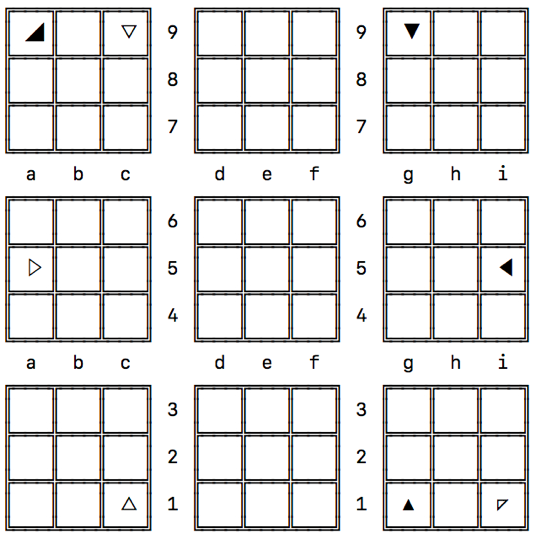
\includegraphics[width=0.5\textwidth]{Imagem1.png}
    \caption{Representation of the initial board.}
    \label{fig:initial-state}
\end{figure}

To update the board we use assert and retract predicates:
\begin{minted}{prolog}
    retract(board(Line,Column,Piece),
    assert(board(Line, Column, NewPiece),
    !.
\end{minted}



\begin{figure}[H]
    \centering
    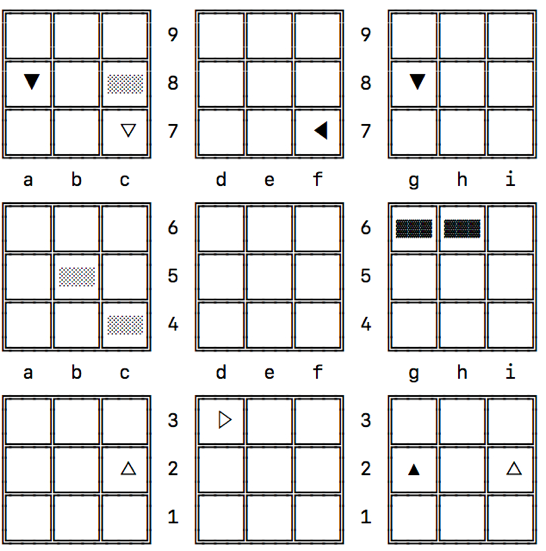
\includegraphics[width=0.5\textwidth]{Imagem2.png}
    \caption{Representation graphic of an intermediate board}
    \label{fig:intermediate-state}
\end{figure}


\vspace{10mm}

%%%%%%%%%%%%%%%%%%%%%%%%%%
\subsection{Board Visualization} 
To represent all different states of all positions on the board, we use the following structure:

\begin{center}
\textbf{N\_Direction}
\end{center}

\textbf{N:} Is the number of player occupying the position.  Can be: 1 or 2.

\textbf{Direction:} Is the direction that the piece is turned to. Can be: n, s, e, w, ne, se, nw, ne.


\vspace{5mm}
\textbf{Note:}  If the position belongs to a player but he hasn’t a piece in that position, the representation is only the number of the player.

\vspace{5mm}

To display the board, it's called the function 'show\_board' that uses the predicate 'translate' in order to show to user a more interesting visualization. 

\subsection{List of Possible Moves} 
Calling the function \textit{get\_all\_possible\_moves}, it saves a list of lists with all possible moves in a global variable called 'list\_movements'.

\subsection{Movements} 
The player can make one move in a direction in front or 45-degrees to the left or right. In each move the player can move form 1 to the number of tiles of his color in that quadrant.

\begin{itemize}
\item \textit{move\_piece(+PLAYER, +LINE, +COLUMN)}

\vspace{5mm}

\textbf{PLAYER} – what player will move a piece.

\textbf{LINE} – the line to where the piece will go.

\textbf{COLUMN} – the column to where the piece will go.

\vspace{5mm}

When the player goes to another quadrant, he can choose to change his direction to 45 degrees to the left ,45 degrees to the right or continue in the same direction.

\vspace{5mm}

\item \textit{quadrant\_change\_direction(+PLAYER, +LINE, +COLUMN, -DIR\_TO\_MOV)}

\vspace{5mm}

\textbf{PLAYER} – what player just got across a quadrant.

\textbf{LINE} – the line to where the piece will go.

\textbf{COLUMN} – the column to where the piece will go.

\textbf{DIR\_TO\_MOV} – in what direction the player wants the piece to stay after crossing to another quadrant.
\end{itemize}

\subsection{Game Ends}
The game will end, 1 round after one of the players run out of
possible movements. Our code for that:

\begin{minted}{prolog}
final:-
    get_all_possible_moves,
    nb_getval(list_movements, MOVES),
    length(MOVES, TAM),
    (TAM == 0 ->
        true
        ;
        nb_getval(player, PLAYER),
        nb_getval(plays_left, PLAYS),
        number_possible_moves_player(PLAYER, COUNT),
        ( COUNT == 0 ->
            ( PLAYS == 0 ->
                true
                ;
                P is PLAYS - 1,
                nb_setval(plays_left, P),
                change_player,
                false
            )
            ;
            false
        )
    ),
    !.

\end{minted}

\subsection{Computer Move} 
The Computer's move is basically a random, although, it's move is tested to make sure that it doesn't make any impossible move. Computer has 3 decision:
\vspace{5mm}

\textit{bot\_choose\_piece(+PLAYER, +LINE, +COLUMN)}

\textit{bot\_choose\_position\_to\_mov(+LINE\_A, +COLUMN\_A, +LINE1, +COLUMN1)}

\textit{bot\_change\_direction(+DIR, +DIR1, +DIR2, -DIR\_TO\_MOV)}

\vspace{10mm}
%%%%%%%%%%%%%%%%%%%%%%%%%%

\section{User Interface}

\begin{figure}[H]
    \centering
    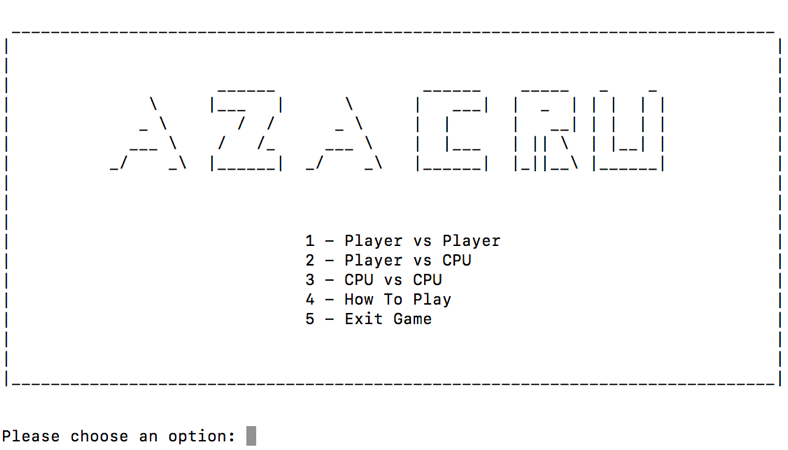
\includegraphics[width=0.5\textwidth]{Imagem3.png}
    \caption{Main Menu Interface}
    \label{fig:i1}
\end{figure}

\begin{figure}[H]
    \centering
    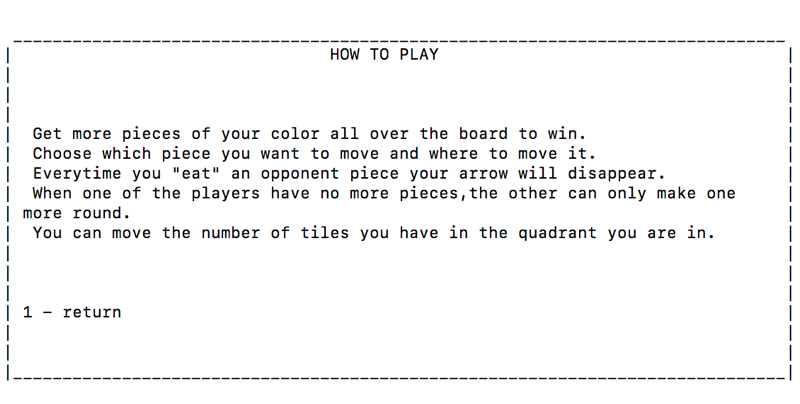
\includegraphics[width=0.5\textwidth]{Imagem4.png}
    \caption{How to Play}
    \label{fig:i2}
\end{figure}

\begin{figure}[H]
    \centering
    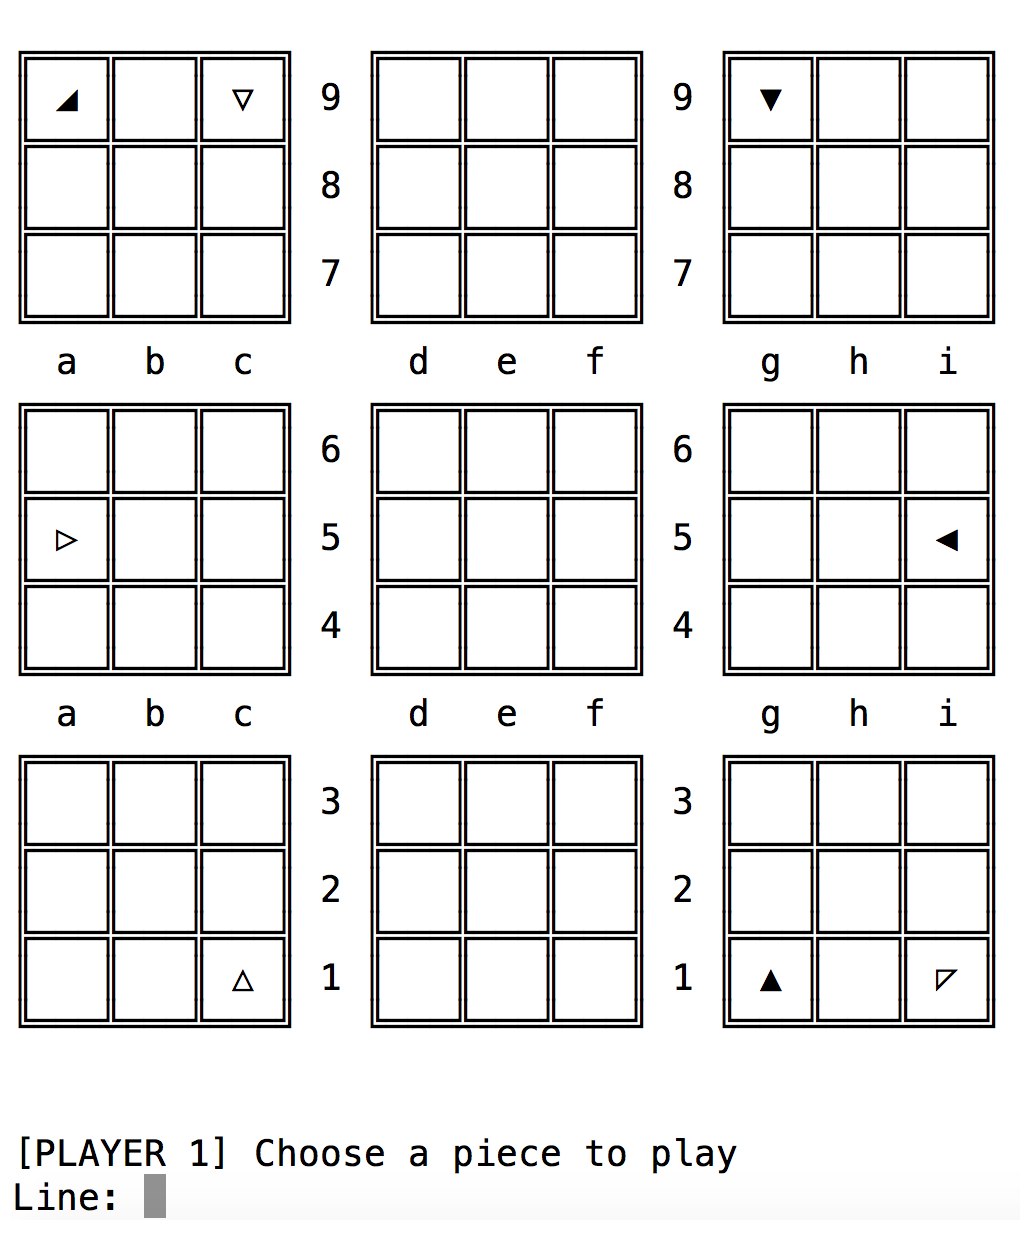
\includegraphics[width=0.5\textwidth]{Imagem5.png}
    \caption{Choose Line}
    \label{fig:i3}
\end{figure}

\begin{figure}[H]
    \centering
    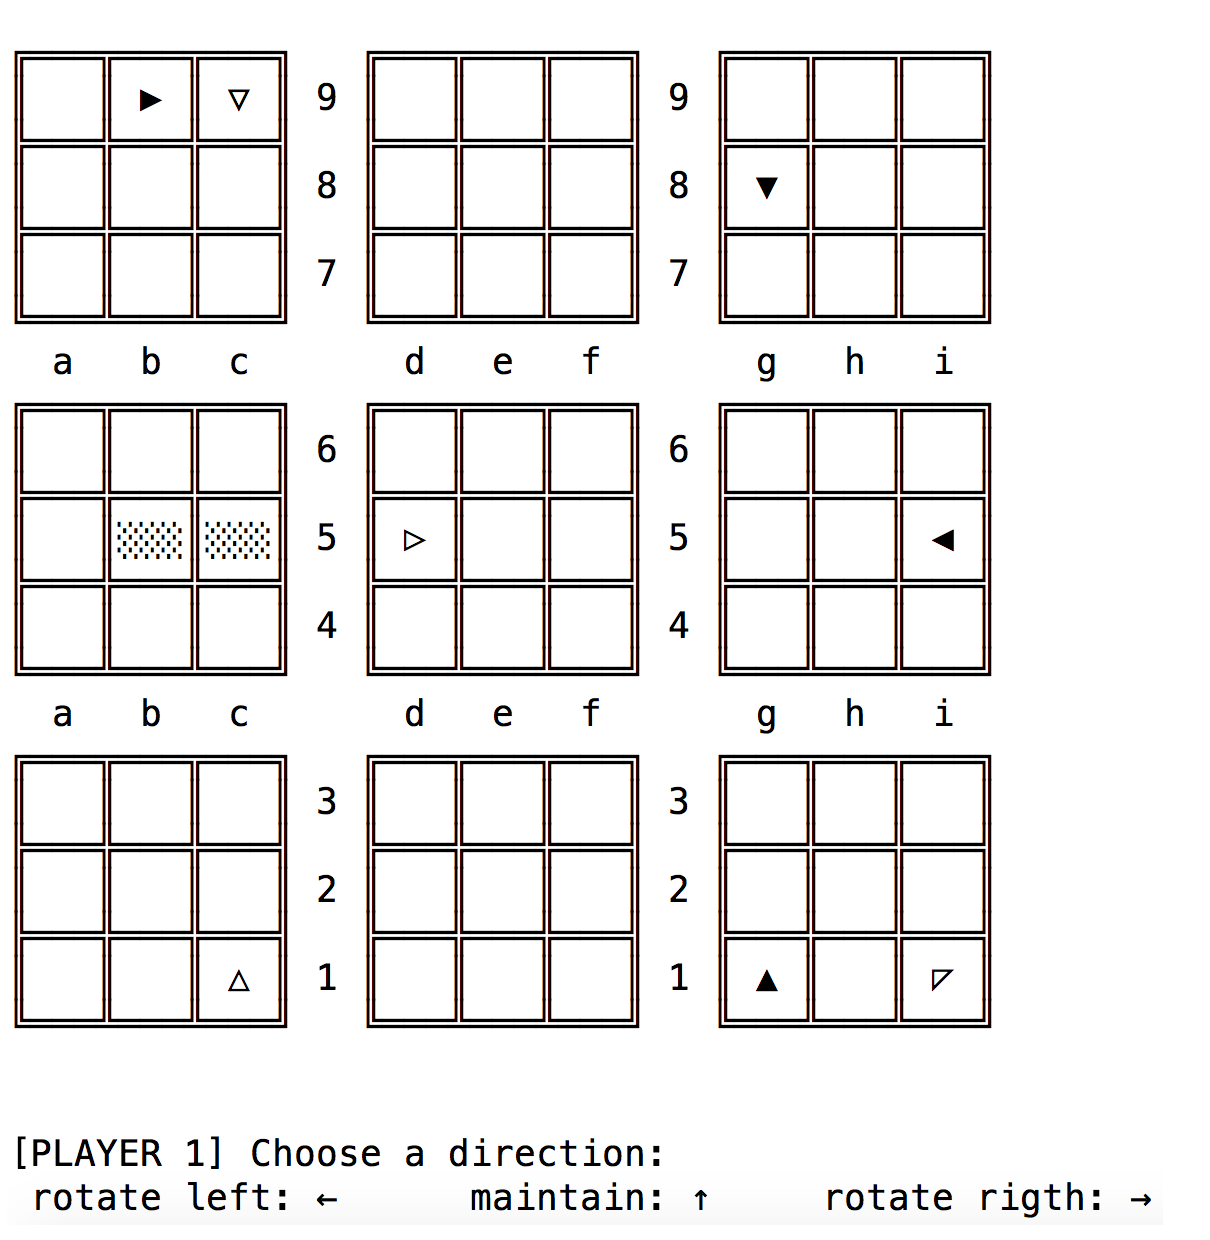
\includegraphics[width=0.5\textwidth]{Imagem6.png}
    \caption{Choose Direction}
    \label{fig:i4}
\end{figure}

\vspace{10mm}
%%%%%%%%%%%%%%%%%%%%%%%%%%
\section{How To Play}
The game must be ran in the terminal with SWI-Prolog. It's not recommend the use of the application SWI-Prolog because the board will be desconfigured, since we use special characters. 

We use macOS to build the game so it's expected some desconfiguration when switching to Windows.
To Run open swipl in the terminal, azacru.pl in the swipl terminal and then use the command 'azacru.'.



\vspace{10mm}
%%%%%%%%%%%%%%%%%%%%%%%%%%
\section{Conclusions}
This Project allowed both members to learn more about Prolog and it's structure.

Every functionality of the game Azacru was incorporated in the most simplified way that was possible with predicates and functions of easy comprehension.

 Although, there was a functionality that could be improved. This functionality was the bot movement that instead of simple random could have a more complexed artificial intelligence so that we would 'think' it's moves so that would be more difficult to the player.



\clearpage
\addcontentsline{toc}{section}{bibliography}
\renewcommand\refname{Bibliography}
\bibliographystyle{plain}
\bibliography{myrefs}


\end{document}
